\section{Конструкторский раздел}

\subsection{Схема базы данных}

\begin{itemize}
    \item Users --- таблица с данными о пользователях.
    \item Projects --- таблица с основными данными о проектах.
    \item ProjectSchemas --- таблица с данными о схемах проектов.
    \item ProjectGrants --- таблица с данными о возможности пользователей размечать данные проектов.
    \item Tasks --- таблица с данными о элементах выборки
    \item LabeledTasks --- таблица с данными о метках
    \item Sessions --- таблица с данными о сессиях пользователей
\end{itemize}

\begin{figure}[h!]
    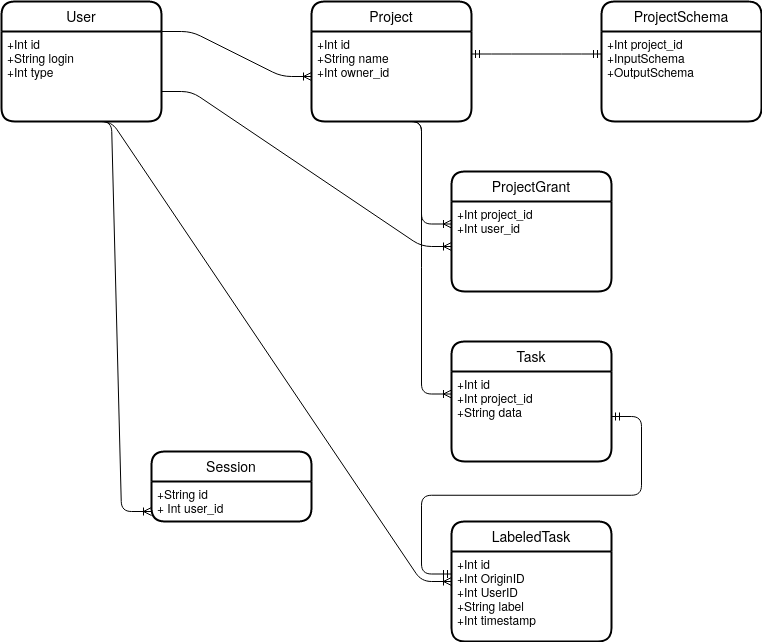
\includegraphics[width=0.9\textwidth]{./dbschema.png}
    \caption{Схема базы данных}
\end{figure}

\subsection{Диаграмма классов доступа к данным}

Данная диаграмма описывает отношения между классами в компоненте доступа к данным.
Для каждой таблицы БД был выделен базовый класс и классы реализации:

\begin{itemize}
    \item Repo --- базовый класс для доступа к данным определенной сущности.
    \item TarantoolRepo --- реализация базового класса Repo для доступа к данным сущности в БД Tarantool.
\end{itemize}

\begin{figure}[h!]
    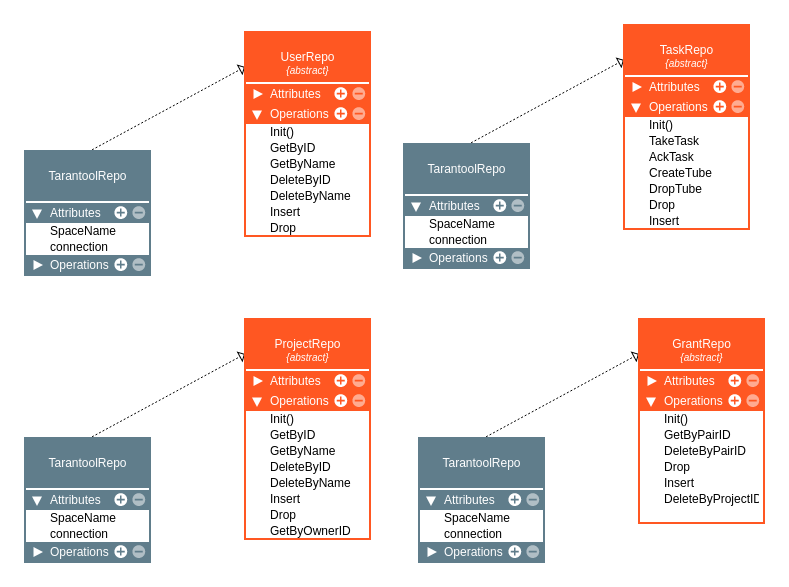
\includegraphics[width=0.9\textwidth]{./dataaccess.png}
    \caption{Диаграмма классов доступа к данным}
\end{figure}


\subsection{Диаграмма классов компоненты бизнес-логики}

Данная диаграмма описывает отношение между
классами в компоненте бизнес-логики.

\begin{itemize}
    \item BaseManager --- базовый класс для менеджеров бизнес-логики. 
        Предоставляет основной интерфейс высокоуровневого доступа 
        к данным модели.

    \item SimpleManager --- реализация базового класса BaseManager, использующая заданную стратегию выполнения бизнес-логики
\end{itemize}


\begin{figure}[h!]
    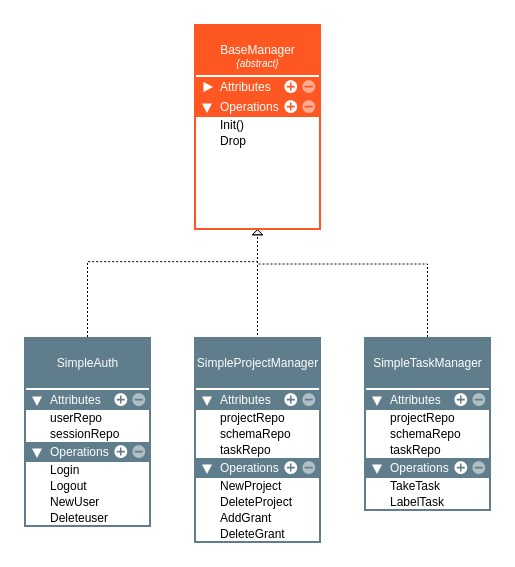
\includegraphics[width=0.7\textwidth]{./business.png}
    \caption{Диаграмма классов бизнес-логики}
\end{figure}

\subsection{Диаграмма классов схем проектов}

Для обеспечения гибкости добавления и выбора различных входных и выходных схем проектов была разработана следующая иерархия классов.

\begin{itemize}
    \item InputSchema --- базовый класс, определяющий возможные значения входных данных
    \begin{itemize} 
        \item ImageSchema --- класс для входных данных в виде изображений
        \item TextSchema --- класс для входных данных в виде текста
        \item TableSchema --- класс для входных данных в виде таблицы
    \end{itemize}
    \item OutputSchema --- базовый класс, определяющий возможные значения выходных данных
    \begin{itemize}
        \item ClassSchema --- класс для выходных данных в виде выбора из заданнах классов
        \item TextSchema --- класс для выходных данных в виде текста
        \item IntegerSchema -- класс для выходных данных в виде целого числа
        \item FloatSchema --- класс для выходных данных в виде числа с плавающей запятой.
    \end{itemize}
\end{itemize}

\begin{figure}[h!]
    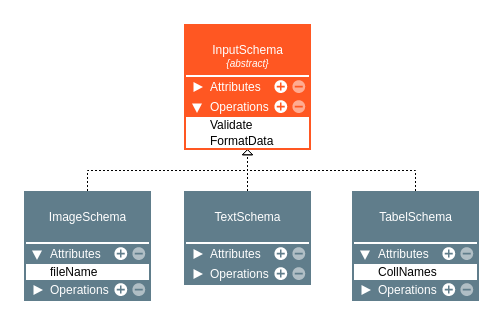
\includegraphics[width=0.9\textwidth]{./inputschema.png}
    \caption{Диаграмма классов входных схем}
\end{figure}

\begin{figure}[h!]
    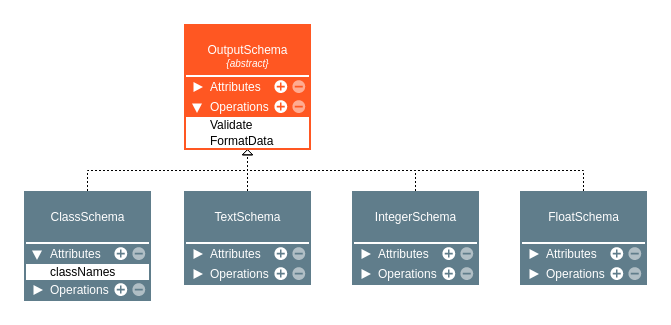
\includegraphics[width=0.9\textwidth]{./outputschema.png}
    \caption{Диаграмма классов выходных схем}
\end{figure}
